\documentclass[11pt,letterpaper]{article}

\usepackage[T1]{fontenc}
\usepackage{mathpazo}
\usepackage{microtype}
\usepackage[margin=1in]{geometry}
\usepackage{amssymb}
\usepackage{tikz}
\usetikzlibrary{arrows.meta,positioning,calc,shapes.geometric,backgrounds,fit}
\usepackage{titlesec}
\usepackage{fancyhdr}
\usepackage{booktabs}
\usepackage{tabularx}
\usepackage{hyperref}

\definecolor{accent}{HTML}{2E4057}
\definecolor{midgray}{HTML}{6B7280}
\definecolor{teal}{HTML}{0D7377}
\definecolor{lightgray}{HTML}{F3F4F6}
\definecolor{darkgray}{HTML}{374151}

\hypersetup{colorlinks=true, linkcolor=teal, urlcolor=teal, citecolor=accent}

\pagestyle{fancy}
\fancyhf{}
\fancyhead[R]{\small\textit{Podcast Infrastructure Research}}
\fancyfoot[C]{\thepage}
\renewcommand{\headrulewidth}{0pt}

\titleformat{\section}[hang]{\Large\bfseries\color{accent}}{}{0pt}{}[\vspace{6pt}]
\titleformat{\subsection}[hang]{\large\bfseries\color{darkgray}}{}{0pt}{}[\vspace{4pt}]
\titleformat{\subsubsection}[hang]{\normalsize\bfseries\color{darkgray}}{}{0pt}{}[\vspace{3pt}]

\title{\textbf{\Large Automated Podcast Infrastructure}\\[8pt]\large From Recording to Publication\\[12pt]\normalsize A Research Survey for the Theseus Media Faculty}
\author{Theseus Intellectual Capital Partners}
\date{April 2026}

\begin{document}

\maketitle

\section*{A Reader's Guide}

\noindent You want to record a conversation and have everything else happen automatically—cleanup, transcription, publishing, and feeding the ideas into your knowledge system. This paper surveys exactly how to build that.

The goal is simple: \textit{the founders sit down, have a philosophical conversation, and walk away}. Everything else—recording backup, noise removal, speaker identification, show notes, chapter markers, publication across dozens of platforms, ingestion into the knowledge graph—should happen automatically or with at most one human approval checkpoint.

This used to be a pipe dream. In 2026, it's achievable. The tools exist. The APIs exist. What doesn't exist is a single platform that glues them all together—so this document is your guide to understanding the gaps and building that glue.

We'll cover:
\begin{itemize}
  \item \textbf{Recording:} Remote and in-studio setups with multi-track audio capture.
  \item \textbf{Transcription:} Speaker identification, accuracy, and the philosophical vocabulary problem.
  \item \textbf{Audio post-production:} Cleanup, noise reduction, loudness normalization.
  \item \textbf{Metadata generation:} Show notes, chapters, and standards-compliant podcast metadata.
  \item \textbf{Publishing:} Distribution to Apple, Spotify, and other platforms via APIs.
  \item \textbf{Knowledge integration:} Feeding the transcript into your internal knowledge graph.
  \item \textbf{Cost and scaling:} Real numbers for different volumes.
\end{itemize}

\noindent By the end, you'll understand the full pipeline, know exactly which tools to use and why, and have concrete code examples for integrating them.

\vspace{12pt}

\section{Recording: Capturing Multi-Track Audio}

\subsection{Why Multi-Track Matters}

When two or three people talk simultaneously, or one person speaks while another is thinking, a single mixed audio file makes it nearly impossible to separate the voices afterward. But if each speaker's audio is recorded on a separate track on their own machine, post-production becomes dramatically simpler: you have clean, isolated sources for transcription, speaker identification, and individual voice-level adjustment.

Modern remote recording platforms and hardware devices all support this. The founders never see it—they just record normally—but the infrastructure is working for them.

\subsection{Remote Recording Platforms}

\subsubsection{Riverside.fm}

Riverside records each participant's audio locally on their machine, then uploads to cloud storage. This means even if the internet connection drops, the local recording is perfect. Riverside released significant API updates in 2025; the REST API v3 (Business tier, \$99/month) allows you to:

\begin{itemize}
  \item List and retrieve completed recordings
  \item Download raw files in WAV, M4A, or MP4 format
  \item Manage sessions and participants
  \item Retrieve metadata including speaker names and track assignments
\end{itemize}

The API cannot start a recording remotely—the founder still presses a button—but everything after recording completion can be fully automated.

\textbf{Latency:} Files are available via API within 2–5 minutes of session completion.

\textbf{Audio quality:} 48 kHz, 16-bit or higher, separate track per participant. Supports video recording as well.

\textbf{Example API call (retrieve recordings):}
\begin{verbatim}
curl -H "Authorization: Bearer YOUR_TOKEN" \
  https://api.riverside.fm/v3/recordings \
  | jq '.[] | {id, title, created_at}'
\end{verbatim}

\subsubsection{SquadCast}

SquadCast (now owned by Descript) records locally per participant and integrates directly with Descript. Once the recording completes, it appears in Descript's editor ready to use. This is the tightest recording-to-editing loop available, but it's less API-friendly than Riverside. There is no public REST API for programmatic episode creation or download—integration is through Descript's native interface only.

\textbf{Cost:} Free with a Descript subscription (\$12–24/month depending on tier).

\subsubsection{Zencastr}

Zencastr records separately per participant and can auto-export to Dropbox or Google Drive via webhook. However, there is no documented API for programmatic integration. Useful if you're already using Dropbox but less automation-friendly than Riverside.

\subsection{In-Person Hardware}

For founders in the same room, you have two good options:

\subsubsection{Zoom PodTrak P4}

A simple four-channel USB mixer (\$200) with XLR inputs, recording to four separate tracks via USB to any computer. Portable, sturdy, and includes basic automation features. The Zoom PodTrak can be controlled via MIDI, allowing tight integration with OBS Studio for scene switching and recording control.

\textbf{Audio quality:} 48 kHz, 24-bit.

\subsubsection{Rodecaster Pro 2}

A higher-end all-in-one mixer (\$600+) with MIDI triggers, onboard recording, and tight integration with streaming and podcast software. Internally records a stereo mix; for true multi-track capture, route USB audio into OBS Studio using BlackHole (macOS) or VB-Cable (Windows) virtual audio drivers.

\subsubsection{OBS Studio}

OBS can be controlled programmatically via WebSocket API:

\begin{itemize}
  \item Start/stop recording
  \item Switch scenes and sources
  \item Adjust audio levels per track
  \item Monitor streaming/recording state
\end{itemize}

This makes OBS the backbone of any fully automated local setup. A Python client library is available.

\textbf{Example (start recording via OBS WebSocket):}
\begin{verbatim}
import json
import websocket

ws = websocket.create_connection(
    "ws://localhost:4455"
)
ws.send(json.dumps({
    "requestType": "StartRecord"
}))
\end{verbatim}

\subsection{Recording Best Practices for Epistemological Discussions}

Even with perfect tools, garbage-in produces garbage-out. Here are practical guidelines for founders:

\subsubsection{Room Acoustics}

\begin{itemize}
  \item \textbf{Avoid hard surfaces.} A bare concrete or tile room creates reflections and echo. Carpets, curtains, and bookshelves absorb sound.
  \item \textbf{Position the microphone 6–8 inches from the mouth,} slightly off-axis to reduce plosives ("p" and "b" sounds).
  \item \textbf{Use a pop filter} if you have one; it's not essential but helps.
  \item \textbf{Minimize background noise.} Close windows, turn off fans, silence phones.
\end{itemize}

\subsubsection{Microphone Technique}

For philosophical conversation, consistent distance and level are more important than fancy gear.

\begin{itemize}
  \item \textbf{Maintain consistent distance} from the microphone throughout the conversation.
  \item \textbf{Speak clearly and directly} into the mic—don't shout, but don't mumble.
  \item \textbf{If one speaker is much louder than another,} adjust input levels in your recording software (or in the hardware mixer) before pressing record.
\end{itemize}

\subsubsection{Recording Format}

Always record to lossless format (WAV or AIFF). Lossy formats (MP3, AAC) discard information that you cannot recover later. Storage is cheap; audio quality is forever.

\subsubsection{Why Multi-Track Matters (Reprise)}

If both founders are on separate channels, you can:
\begin{itemize}
  \item Adjust each speaker's level independently in post-production.
  \item Run speaker identification and transcription on each track separately, then merge.
  \item Remove background noise from one speaker without affecting the other.
\end{itemize}

\subsection{Recommendation}

For Theseus:

\begin{itemize}
  \item \textbf{Remote sessions:} Riverside.fm (API-accessible, multi-track, cloud backup).
  \item \textbf{In-person sessions:} Zoom PodTrak P4 + OBS Studio (portable, multi-track, scriptable).
\end{itemize}

Both produce separate WAV files per speaker. Configure auto-upload to S3 or a watched folder to trigger the downstream pipeline.

\vspace{12pt}

\section{Transcription: Converting Audio to Text with Speaker Labels}

\subsection{Why Speaker Labels Matter}

A transcript without speaker names is nearly useless: "Um, I think that's epistemologically problematic. On the other hand, consider..." Who said that? Who is responding? For philosophical discourse, attribution is essential—you need to know which founder articulated which idea so you can trace the provenance of concepts through your knowledge graph.

Modern transcription services can identify different speakers and label them automatically. This is called \textit{diarisation} (or speaker diarization in American English).

\subsection{API Services: Current Landscape (2025–2026)}

\subsubsection{OpenAI GPT-4o Transcribe}

As of early 2025, OpenAI's GPT-4o Transcribe model includes native speaker diarisation at \$0.006 per minute. This is the same price as base Whisper but with \textit{significantly lower word error rates} and built-in speaker labels.

\begin{itemize}
  \item \textbf{Word Error Rate (WER):} 4–6\% on academic speech (excellent).
  \item \textbf{Diarisation accuracy:} ~95\% on 2–4 speakers.
  \item \textbf{Processing time:} ~30 seconds for a 1-hour file (via API).
  \item \textbf{API access:} Yes, via OpenAI API with simple JSON requests.
\end{itemize}

\textbf{Example usage (Python):}
\begin{verbatim}
import openai

with open("episode.m4a", "rb") as audio:
    transcript = openai.Audio.transcribe(
        model="gpt-4o-turbo",
        file=audio,
        language="en"
    )

for segment in transcript.get("segments", []):
    print(f"{segment['speaker']}: {segment['text']}")
\end{verbatim}

\subsubsection{Deepgram Nova-3}

Deepgram is the cost leader at scale: \$0.0077 per minute pay-as-you-go, dropping to \$0.003/min above 1,000 hours/month. Diarisation is included at no extra charge. Both real-time and batch modes are supported.

\begin{itemize}
  \item \textbf{Strength:} Excellent for volume; lowest per-minute cost at scale.
  \item \textbf{Weakness:} Slightly less accurate on academic vocabulary; no built-in term injection.
  \item \textbf{Processing time:} Real-time streaming or batch, ~15 seconds for 1-hour file.
\end{itemize}

\subsubsection{AssemblyAI}

AssemblyAI has the best diarisation tooling: 2.9\% speaker count error rate, prompted diarisation (you can tell it "Speaker A is Michael, Speaker B is Jane"), and entity detection that identifies mentioned thinkers, organisations, and concepts.

\begin{itemize}
  \item \textbf{Strength:} Best speaker identification; can accept speaker names as hints.
  \item \textbf{Requirement:} Each speaker must produce 30+ seconds of continuous, uninterrupted speech for accurate labelling. In a true dialogue, this can be tricky.
  \item \textbf{Cost:} \$0.0083/min. Streaming API available for real-time processing.
\end{itemize}

In 2025, AssemblyAI launched their "Universal" streaming model with built-in diarisation and is probably the best option for real-time transcription during recording.

\subsubsection{Amazon Transcribe}

Amazon Transcribe has the strongest custom vocabulary support: you can upload a vocabulary file with domain-specific terms ("Lakatos," "Feyerabend," "falsifiability," "epistemology"), and even train custom language models for significant accuracy gains.

\begin{itemize}
  \item \textbf{Strength:} Custom vocabulary, custom language models.
  \item \textbf{Cost:} \$0.0001 per second (\$0.006/min), similar to Whisper.
  \item \textbf{Limitation:} Diarisation available only in batch mode; no real-time streaming.
\end{itemize}

\subsubsection{Google Cloud Speech-to-Text v2 (Chirp 3)}

Supports diarisation but only in batch mode, not streaming. At \$0.016/minute, it is the most expensive option and offers no clear advantage over Whisper, Deepgram, or AssemblyAI for this use case.

\subsubsection{Apple SpeechAnalyzer (WWDC 2025)}

Apple released SpeechAnalyzer at WWDC 2025, which processes audio extremely fast on-device (local inference). Requires macOS 15+. No network request; all processing happens on the Mac. If you're already in the Apple ecosystem, this is worth exploring, but it doesn't have a documented public API yet for enterprise use.

\subsection{Self-Hosted Options}

\subsubsection{WhisperX}

WhisperX combines:
\begin{itemize}
  \item \textbf{faster-whisper:} OpenAI's Whisper model accelerated 70x via CTranslate2 (quantization + batch processing).
  \item \textbf{Word-level forced alignment:} Precise timing for each word, not just each segment.
  \item \textbf{pyannote.audio:} Speaker diarisation via neural speaker embeddings.
\end{itemize}

Runs on any NVIDIA GPU with 8GB+ VRAM. At Theseus's volume (perhaps 8 hours/month), self-hosting costs roughly \$0.30–\$1.00/day on a cloud GPU (via Runpod or Lambda Labs)—comparable to or cheaper than API costs, with the advantage of keeping all transcript data on-premises.

For 8 hours/month:
\begin{itemize}
  \item API cost (GPT-4o): \$36/year
  \item Self-hosted GPU cost: \$108–300/year
\end{itemize}

At this volume, API is cheaper. But if you prioritize data privacy or plan to scale to 50+ hours/month, self-hosting becomes more attractive.

\subsubsection{faster-whisper (without diarisation)}

faster-whisper alone (without speaker identification) runs comfortably on a MacBook Pro with Apple Silicon, processing audio at 10–20x real-time on the large-v2 model. This is a good option if you don't need speaker labels, but for Theseus, speaker identification is essential.

\subsection{The Vocabulary Problem}

Standard transcription services will misspell or garble philosophical terminology:

\begin{itemize}
  \item "Polanyi" becomes "Polani"
  \item "Feyerabend" becomes "Fireman"
  \item "epistemological" becomes "epidemiological"
  \item "Kuhn" becomes "Coon"
\end{itemize}

Two mitigations:

\textbf{(1) Custom vocabulary files} (supported by Amazon Transcribe and Deepgram). Upload a JSON file listing terms you expect to hear:

\begin{verbatim}
{
  "phrases": [
    "Polanyi", "Feyerabend", "falsifiability",
    "epistemology", "Lakatos", "Kuhn", "Popper"
  ]
}
\end{verbatim}

\textbf{(2) Post-transcription LLM correction pass.} After transcription, send the transcript to GPT-4 or Claude with a reference list of expected terms and a simple prompt: "Correct any misspellings of the following terms: [list]. Return the corrected transcript."

The second approach is simpler to implement and highly effective. It's also language-agnostic—works for any transcript, not just those using a specific transcription service.

\subsection{Latency Benchmarks}

\begin{center}
\begin{tabular}{lrr}
\toprule
\textbf{Service} & \textbf{Time for 1h Audio} & \textbf{Cost} \\
\midrule
GPT-4o Transcribe (API) & 30s & \$0.36 \\
Deepgram Nova-3 (batch) & 15s & \$0.0077/min \\
AssemblyAI (batch) & 45s & \$0.0083/min \\
Amazon Transcribe & 60–120s & \$0.006/min \\
WhisperX (GPU) & 180–300s & \$0.30–1.00 \\
\bottomrule
\end{tabular}
\end{center}

For context: a 1-hour episode costs \$0.36 on GPT-4o Transcribe, or about \$3.50/month at one episode per week.

\subsection{Recommendation}

Use \textbf{OpenAI GPT-4o Transcribe} for primary transcription. It offers the best combination of accuracy, diarisation quality, and cost. Then add a \textbf{post-transcription LLM pass} that corrects philosophical terminology against a curated vocabulary list.

At 8 hours/month, total transcription cost is approximately \$3/month.

If you need real-time transcription during recording (to generate show notes immediately), use \textbf{AssemblyAI's streaming API} or \textbf{Apple SpeechAnalyzer}.

\vspace{12pt}

\section{Speaker Diarization Deep Dive}

\subsection{Why Diarization Matters for Knowledge Graphs}

In a traditional podcast, you know who is speaking because you can hear the voice. But when feeding a transcript into a knowledge graph, you need explicit speaker labels so you can attribute claims, ideas, and arguments to specific people. "That argument reminds me of what Michael said in episode 7 about falsifiability"—this only works if the transcript says "Michael: ..." not just "...".

Diarization is the automatic identification of speaker boundaries and labels.

\subsection{Methods}

\subsubsection{API-Based Diarization}

All major transcription services include diarization. The accuracy depends on:

\begin{itemize}
  \item \textbf{Number of speakers:} 2–3 speakers is easier than 4+.
  \item \textbf{Speaking patterns:} Long, uninterrupted turns are easier to label than rapid back-and-forth.
  \item \textbf{Audio quality:} Clean, multi-track audio makes diarization trivial.
  \item \textbf{Speaker hints:} If you tell the system "Speaker 1 is Michael, Speaker 2 is Jane," accuracy improves.
\end{itemize}

\subsubsection{pyannote.audio}

A PyTorch-based open-source speaker diarization library. Works by:

\begin{enumerate}
  \item \textbf{Speaker embedding:} Extract a learned vector representation of each speaker's voice.
  \item \textbf{Clustering:} Group similar embeddings into speakers.
  \item \textbf{Segmentation:} Find speaker boundaries in the audio timeline.
\end{enumerate}

Accuracy: ~90–95\% on 2–4 speakers. Runs locally, requires NVIDIA GPU (8GB+), but free and open-source.

Usage with WhisperX:

\begin{verbatim}
from whisperx import load_model, transcribe

model = load_model("large-v2",
                    device="cuda",
                    compute_type="float16")
result = transcribe(model, "episode.m4a")

# Apply diarization
diarize_model = load_model("pyannote/speaker-diarization",
                           device="cuda")
diarization = diarize_model({"uri": "blah",
                             "audio": "episode.m4a"})
\end{verbatim}

\subsection{Accuracy Comparison}

\begin{center}
\begin{tabular}{lcc}
\toprule
\textbf{Method} & \textbf{2–3 Speakers} & \textbf{Cost (per 1h)} \\
\midrule
GPT-4o Transcribe & 95\%+ & \$0.36 \\
AssemblyAI & 94\%+ & \$0.50 \\
Deepgram Nova-3 & 90\% & \$0.46 \\
Amazon Transcribe & 88\% & \$0.36 \\
pyannote.audio & 88\% & \$0.50 (GPU) \\
\bottomrule
\end{tabular}
\end{center}

GPT-4o is the best in accuracy and cost. If you have 4+ speakers or rapid turn-taking, use AssemblyAI with speaker hints.

\subsection{Failure Modes and Fallbacks}

\subsubsection{Failure Mode: Indistinguishable Speakers}

If two founders have very similar voices or similar speaking styles, diarization may confuse them.

\textbf{Fallback:} Provide speaker hints to the transcription service. "Speaker 1 is Michael (male), Speaker 2 is Jane (female)." Also consider recording each speaker on a separate microphone track—this makes diarization trivial.

\subsubsection{Failure Mode: Long Monologues}

If one speaker goes on for 5+ minutes uninterrupted, diarization is unnecessary but harmless—it just labels the whole segment as one speaker.

\subsubsection{Failure Mode: Background Speakers}

If a third person is audible in the background, the diarization model may try to identify them as a speaker. Minimize this by controlling the recording environment.

\vspace{12pt}

\section{Audio Post-Production: Cleanup, Normalization, Assembly}

\subsection{The Cleanup Pipeline}

After transcription, the raw audio needs:

\begin{enumerate}
  \item \textbf{Noise reduction:} Remove background hum, HVAC, ambient noise.
  \item \textbf{Normalization:} Equalize levels between speakers (one speaker naturally louder than another).
  \item \textbf{Equalization:} Smooth out harsh frequencies, improve clarity.
  \item \textbf{Loudness normalization:} Ensure the final episode meets podcast distribution standards.
\end{enumerate}

\subsection{Automated Cleanup Tools}

\subsubsection{Auphonic API}

Auphonic is purpose-built for podcast production. It handles loudness normalisation, noise reduction, equalization, and adaptive levelling between speakers. It has a full REST API and webhooks for fully automated workflows.

\textbf{Pricing:} Free tier covers 2 hours/month. After that, pay per millisecond of audio processed. At 2 episodes/week (8 hours/month), you'll pay roughly \$10–30/month depending on processing intensity.

\textbf{API workflow:}

\begin{enumerate}
  \item Upload raw audio to Auphonic API.
  \item Auphonic processes it (noise reduction, levelling, EQ).
  \item Receive the processed audio via webhook or direct download.
  \item Pass to next stage (loudness normalization, assembly).
\end{enumerate}

\textbf{Example (Python):}

\begin{verbatim}
import requests

# Create production
payload = {
    "production": {
        "metadata": {
            "title": "Episode 42"
        }
    }
}
resp = requests.post(
    "https://api.auphonic.com/productions.json",
    json=payload,
    auth=("user@example.com", "password")
)
prod_id = resp.json()["data"]["uuid"]

# Upload file
with open("raw.wav", "rb") as f:
    files = {"input_file": f}
    requests.post(
        f"https://api.auphonic.com/productions/{prod_id}"
        "/upload.json",
        files=files,
        auth=("user@example.com", "password")
    )

# Start processing
requests.post(
    f"https://api.auphonic.com/productions/{prod_id}"
    "/start.json",
    auth=("user@example.com", "password")
)
\end{verbatim}

\subsubsection{Adobe Podcast Enhance Speech}

Produces excellent results for noise removal and speech clarity but is browser-only with no API. Useless for automation.

\subsubsection{iZotope RX}

The gold standard for manual audio restoration (de-reverb, de-click, spectral repair) but is desktop software without API access. Useful as a fallback for problem recordings, not for routine automation.

\subsection{Loudness Normalization and Assembly}

The podcast loudness standard is \textbf{–16 LUFS (integrated loudness)} with a \textbf{–1.5 dBTP true peak limit}. Every major podcast platform enforces this or will normalize your episode to it. FFmpeg handles this natively with a two-pass loudnorm filter.

\textbf{Pass 1 (analyze):}

\begin{verbatim}
ffmpeg -i raw.wav \
  -af "loudnorm=I=-16:TP=-1.5:LRA=7:print_format=json" \
  -f null /dev/null 2>&1 | tail -12
\end{verbatim}

This outputs JSON with measured loudness values.

\textbf{Pass 2 (apply):}

\begin{verbatim}
ffmpeg -i raw.wav \
  -af "loudnorm=I=-16:TP=-1.5:LRA=7:\
  measured_I=-18.2:\
  measured_TP=-2.1:\
  measured_LRA=5.8:\
  measured_thresh=-30.0" \
  -acodec libmp3lame -q:a 5 \
  output.mp3
\end{verbatim}

Intro and outro segments are concatenated using FFmpeg's concat demuxer with optional crossfades:

\begin{verbatim}
# file list.txt
file 'intro.wav'
file 'episode.wav'
file 'outro.wav'

ffmpeg -f concat -safe 0 -i list.txt \
  -af "crossfade=d=2" \
  -acodec libmp3lame -q:a 5 \
  final.mp3
\end{verbatim}

The entire assembly step can be scripted in Python using subprocess calls to FFmpeg. This is free, reliable, and fully under your control.

\subsection{Recommendation}

\begin{itemize}
  \item Use \textbf{Auphonic API} for noise reduction, speaker levelling, and equalization (automated, high quality).
  \item Use \textbf{FFmpeg} for loudness normalisation and audio assembly (free, fully scriptable, part of the pipeline).
  \item Optionally run Descript manually for filler word removal, or build a custom filler-word remover using the transcript as a guide.
\end{itemize}

\vspace{12pt}

\section{Show Notes, Chapters, and Podcast 2.0 Standards}

\subsection{AI-Generated Metadata}

Several tools generate show notes, episode descriptions, chapter markers, and social media content from podcast audio or transcripts:

\begin{itemize}
  \item \textbf{Podsqueeze:} Produces the most useful chapter breakdowns with precise timestamps, blog posts, social media content, and key quotes. Best for structured show notes.
  \item \textbf{Castmagic:} Generates show notes, tweets, blog summaries, and Q\&A sections. Strong on content repurposing.
  \item \textbf{Capsho:} Focuses on marketing: episode titles, descriptions, email newsletters, social content optimised for growth.
\end{itemize}

However, for Theseus, the most effective approach is likely a \textbf{custom LLM pass on the transcript}. Given that the transcript is already available and the firm has specific requirements (philosophical rigour, proper attribution of ideas to specific thinkers), a custom prompt against GPT-4 or Claude that generates show notes, chapter markers, and a 2–3 sentence episode description will produce better results than generic tools. The prompt can reference the firm's vocabulary list and style guidelines.

\textbf{Example prompt:}

\begin{verbatim}
You are a research analyst for Theseus,
an intellectual capital firm focused on
philosophy and epistemology.

Given the following transcript, generate:
1. A 2-3 sentence episode summary
2. 5-7 chapter markers with timestamps
3. A bulleted list of 3-5 key ideas discussed

Transcript:
[transcript here]

Respond in JSON format.
\end{verbatim}

\subsection{Podcast 2.0 Standards}

The Podcast 2.0 namespace (podcastindex.org/namespace/1.0) defines rich metadata tags that modern podcast apps support. This is crucial for discoverability and accessibility.

\subsubsection{podcast:chapters}

Links to an external JSON file containing chapter data with timestamps, titles, optional images, and URLs. Over 500,000 episodes already use this format.

\textbf{JSON format:}

\begin{verbatim}
{
  "version": "1.2.0",
  "chapters": [
    {
      "startTime": 0,
      "title": "Intro",
      "img": "https://example.com/intro.jpg"
    },
    {
      "startTime": 300,
      "title": "The Problem of Induction",
      "img": "https://example.com/ch1.jpg"
    }
  ]
}
\end{verbatim}

\subsubsection{podcast:transcript}

Links to a WebVTT or SRT transcript file, enabling search and accessibility features in supporting apps.

\textbf{WebVTT format:}

\begin{verbatim}
WEBVTT

00:00:00.000 --> 00:00:05.000
Michael: Welcome to Theseus, episode 42.

00:00:05.000 --> 00:00:12.000
Jane: Today we're discussing the problem
of induction in epistemology.
\end{verbatim}

Both can be programmatically generated from the transcript and chapter data, hosted on S3, and linked in the RSS feed.

\subsection{Recommendation}

Generate chapters and metadata using a custom LLM prompt. Host the JSON and WebVTT files on S3. Link them in the Buzzsprout RSS feed using the Podcast 2.0 namespace tags.

\vspace{12pt}

\section{Publishing and Distribution}

\subsection{Hosting Platforms with APIs}

\subsubsection{Buzzsprout}

Buzzsprout has the best-documented podcast hosting API: RESTful, JSON-based, token-authenticated. You can:

\begin{itemize}
  \item Upload episodes (MP3 audio files)
  \item Set metadata (title, description, tags, publication date)
  \item Publish programmatically
  \item Query episode data
\end{itemize}

Buzzsprout then distributes the RSS feed to Apple Podcasts, Spotify, Google Podcasts, and 100+ other directories automatically.

\textbf{Pricing:} \$12/month (basic plan).

\textbf{Example (create and publish episode):}

\begin{verbatim}
import requests

BUZZSPROUT_API_KEY = "YOUR_KEY"
PODCAST_ID = "12345"

# Create episode
payload = {
    "episode": {
        "title": "Episode 42",
        "description": "Discussion of induction",
        "published_at": "2026-04-12T10:00:00Z"
    }
}

resp = requests.post(
    f"https://www.buzzsprout.com/api/podcasts"
    f"/{PODCAST_ID}/episodes",
    json=payload,
    headers={"Authorization": f"Token {BUZZSPROUT_API_KEY}"}
)

episode_id = resp.json()["id"]

# Upload audio
with open("final.mp3", "rb") as f:
    files = {"audio_file": f}
    requests.post(
        f"https://www.buzzsprout.com/api/podcasts"
        f"/{PODCAST_ID}/episodes/{episode_id}",
        files=files,
        headers={"Authorization": f"Token {BUZZSPROUT_API_KEY}"}
    )

# Publish
requests.patch(
    f"https://www.buzzsprout.com/api/podcasts"
    f"/{PODCAST_ID}/episodes/{episode_id}",
    json={"episode": {"published_at": "2026-04-12T10:00:00Z"}},
    headers={"Authorization": f"Token {BUZZSPROUT_API_KEY}"}
)
\end{verbatim}

\subsubsection{Transistor.fm and Podbean}

Transistor.fm and Podbean lack publicly documented APIs for episode creation. Transistor can import from other platforms, but programmatic episode creation requires contacting support.

\subsubsection{Spotify for Podcasters}

Has read-only APIs only—you can query podcast data but cannot publish through the API. Publishing requires RSS feed submission.

\subsection{Recommendation}

Use \textbf{Buzzsprout} as the publishing hub. Upload the final MP3 + metadata via API. Buzzsprout handles RSS generation and distribution to all major directories. Host Podcast 2.0 chapter and transcript files on S3 and link them in the RSS feed.

\vspace{12pt}

\section{The Noosphere Ingestion Pipeline}

\subsection{From Recording to Knowledge Graph}

Podcast audio doesn't exist in isolation. For Theseus, the episode's transcript and metadata must flow into the knowledge graph (Noosphere) so that ideas, thinkers, and arguments are indexed and queryable.

\subsection{Data Flow}

\begin{enumerate}
  \item \textbf{Raw audio} uploaded to S3 (triggered by Riverside webhook or file watch).
  \item \textbf{Transcription} via GPT-4o Transcribe + speaker labels.
  \item \textbf{Post-transcription correction} using LLM pass with vocabulary list.
  \item \textbf{Chapter generation} using LLM prompt.
  \item \textbf{Metadata assembly:} JSON chapters, WebVTT transcript, RSS feed entry.
  \item \textbf{Noosphere ingestion:} Feed the transcript, chapters, and episode metadata into the knowledge graph.
\end{enumerate}

\subsection{Integration with Noosphere}

The Noosphere ingestion endpoint accepts JSON with:

\begin{verbatim}
{
  "source": "podcast",
  "episode_id": "42",
  "title": "The Problem of Induction",
  "speakers": ["Michael", "Jane"],
  "transcript": "Michael: Welcome...",
  "chapters": [...],
  "publication_date": "2026-04-12",
  "audio_url": "https://..."
}
\end{verbatim}

This data is indexed such that:

\begin{itemize}
  \item Ideas and thinkers mentioned are extracted and linked.
  \item Claims are attributed to speakers.
  \item The transcript is searchable.
  \item Connections to other episodes and sources are inferred.
\end{itemize}

\subsection{Celery Task for Ingestion}

\begin{verbatim}
from celery import shared_task
import requests

@shared_task
def ingest_to_noosphere(episode_id,
                        transcript,
                        chapters):
    payload = {
        "source": "podcast",
        "episode_id": episode_id,
        "transcript": transcript,
        "chapters": chapters
    }

    resp = requests.post(
        "https://noosphere.example.com/ingest",
        json=payload,
        auth=("api_user", "api_key")
    )

    return resp.json()
\end{verbatim}

\vspace{12pt}

\section{Cost Analysis Deep Dive}

The total cost depends on episode length and publication frequency. Here's a detailed breakdown:

\subsection{Scenario 1: 1 Episode per Week (52 episodes/year, 52 hours)}

\begin{center}
\begin{tabular}{lrr}
\toprule
\textbf{Component} & \textbf{Annual Cost} & \textbf{Notes} \\
\midrule
Recording (Riverside Business) & \$99–0 & or free (OBS + PodTrak) \\
Transcription (GPT-4o) & \$19 & 3,120 min/year \\
Audio cleanup (Auphonic) & \$0–30 & free tier suffices \\
LLM passes (metadata) & \$10–25 & GPT-4o \\
Audio assembly (FFmpeg) & \$0 & free \\
Publishing (Buzzsprout) & \$144 & \$12/month \\
Storage (S3) & \$5–10 & minimal \\
Voice cloning (optional) & \$0–120 & ElevenLabs \\
Orchestration (Celery) & \$0 & on existing server \\
\midrule
\textbf{Total} & \textbf{\$277–428} & \\
\bottomrule
\end{tabular}
\end{center}

\subsection{Scenario 2: 2 Episodes per Week (104 episodes/year, 104 hours)}

\begin{center}
\begin{tabular}{lrr}
\toprule
\textbf{Component} & \textbf{Annual Cost} & \textbf{Notes} \\
\midrule
Recording & \$99–0 & \\
Transcription & \$37 & 6,240 min/year \\
Audio cleanup & \$0–60 & Auphonic \\
LLM passes & \$20–50 & \\
Audio assembly & \$0 & \\
Publishing & \$144 & \\
Storage & \$10–20 & \\
Voice cloning & \$0–240 & \\
Orchestration & \$0 & \\
\midrule
\textbf{Total} & \textbf{\$310–551} & \\
\bottomrule
\end{tabular}
\end{center}

\subsection{Scenario 3: 4 Episodes per Week (208 episodes/year, 208 hours)}

\begin{center}
\begin{tabular}{lrr}
\toprule
\textbf{Component} & \textbf{Annual Cost} & \textbf{Notes} \\
\midrule
Recording & \$99–0 & \\
Transcription & \$74 & 12,480 min/year \\
Audio cleanup & \$20–120 & Auphonic \\
LLM passes & \$40–100 & \\
Audio assembly & \$0 & \\
Publishing & \$144 & \\
Storage & \$20–40 & \\
Voice cloning & \$0–480 & \\
Orchestration & \$0 & \\
\midrule
\textbf{Total} & \textbf{\$397–894} & \\
\bottomrule
\end{tabular}
\end{center}

\subsection{Notes}

\begin{itemize}
  \item These estimates assume using Riverside for remote recording. Using OBS + PodTrak saves \$99–300.
  \item Auphonic's free tier covers 2 hours/month; beyond that, costs scale with processing time.
  \item LLM costs assume GPT-4o at \$0.005 per 1K input tokens and \$0.015 per 1K output tokens. A 1-hour transcript is ~20K tokens; generating metadata and corrections adds another 5K tokens, totaling ~\$0.13 per episode.
  \item Storage (S3) assumes ~500 MB per episode (raw audio, processed audio, transcripts, metadata).
  \item Voice cloning is entirely optional and is included only for branded episode intros.
\end{itemize}

\vspace{12pt}

\section{Build vs. Buy Decision Matrix}

For each pipeline stage, should you build custom, use an API, or use a platform?

\begin{center}
\begin{tabular}{lccc}
\toprule
\textbf{Stage} & \textbf{Build} & \textbf{API} & \textbf{Platform} \\
\midrule
Recording & \checkmark\checkmark & \checkmark & \checkmark\checkmark \\
Transcription & \checkmark & \checkmark\checkmark & \checkmark \\
Speaker ID & \checkmark & \checkmark\checkmark & \checkmark \\
Audio cleanup & \checkmark & \checkmark\checkmark & \checkmark \\
Loudness norm & \checkmark\checkmark & & \\
Filler removal & \checkmark & & \checkmark \\
Chapters/notes & \checkmark\checkmark & \checkmark & \checkmark \\
Publishing & & \checkmark\checkmark & \checkmark \\
Noosphere ingest & \checkmark\checkmark & & \\
\bottomrule
\end{tabular}
\end{center}

Legend: \checkmark\checkmark = recommended | \checkmark = viable | blank = not recommended

\textbf{Interpretation:}

\begin{itemize}
  \item \textbf{Recording:} Build (Riverside + OBS) or use a platform (Riverside, SquadCast). Don't try to build your own recording infrastructure.
  \item \textbf{Transcription:} Use an API (GPT-4o Transcribe, Deepgram, AssemblyAI). Building is possible (WhisperX) but overkill.
  \item \textbf{Audio cleanup:} Use an API (Auphonic) or build (FFmpeg). Both are viable; Auphonic is simpler.
  \item \textbf{Loudness normalization:} Build with FFmpeg. It's free and reliable.
  \item \textbf{Filler removal:} Build custom or accept manual (Descript). No good API option.
  \item \textbf{Chapters \& metadata:} Build with a custom LLM prompt. More control, better results than generic tools.
  \item \textbf{Publishing:} Use an API (Buzzsprout). Don't build your own podcast hosting.
  \item \textbf{Noosphere ingestion:} Build custom. This is specific to your knowledge graph and cannot be outsourced.
\end{itemize}

\vspace{12pt}

\section{Quality Assurance}

\subsection{Verification Steps}

Before publishing an episode, verify:

\begin{enumerate}
  \item \textbf{Audio quality:} Listen to a 30–60 second sample from the middle of the episode. Check for: noise, distortion, speaker balance.
  \item \textbf{Transcription accuracy:} Spot-check 50–100 words of the transcript. Look for: philosophical term spelling, speaker attribution, major words missed.
  \item \textbf{Metadata correctness:} Verify: episode title, description, chapter timestamps, speaker names.
  \item \textbf{Loudness compliance:} Check that the final MP3 is –16 LUFS. Loudness analysis tools: ffmpeg-normalize, Audacity, or online meters.
\end{enumerate}

\subsection{Automated Quality Checks}

You can automate some of these:

\begin{verbatim}
import subprocess
import json

# Extract loudness
result = subprocess.run([
    "ffmpeg", "-i", "final.mp3",
    "-af", "loudnorm=print_format=json",
    "-f", "null", "/dev/null"
], capture_output=True, text=True)

loudness_data = json.loads(
    result.stderr.split("Summary:")[-1]
)

I = float(loudness_data["integrated_loudness"])
assert abs(I - (-16)) < 0.5,
    f"Loudness {I} outside target range"

# Spot-check transcript
with open("transcript.vtt") as f:
    transcript = f.read()

vocab = ["Polanyi", "Feyerabend", "Kuhn", "Popper"]
missing = [v for v in vocab
           if v not in transcript]

if missing:
    print(f"Warning: {missing} not found in transcript")
\end{verbatim}

\vspace{12pt}

\section{Scaling Considerations}

\subsection{What Changes at Different Volumes?}

\subsubsection{1–2 Episodes per Week}

At this volume, everything is manual-friendly. You can afford to:

\begin{itemize}
  \item Use Riverside for remote sessions (no need to build OBS infrastructure).
  \item Run transcription on-demand via API.
  \item Manually spot-check each episode before publishing.
  \item Keep everything on S3; minimal storage complexity.
\end{itemize}

Cost remains under \$500/year.

\subsubsection{4–8 Episodes per Week}

At this volume, you need:

\begin{itemize}
  \item \textbf{Batch processing:} Process multiple episodes in parallel. Celery task queues become essential.
  \item \textbf{Cost optimization:} Switch to Deepgram for transcription (cheaper at scale than GPT-4o).
  \item \textbf{Storage scaling:} Consider dedicated S3 lifecycle policies (auto-delete raw audio after processing).
  \item \textbf{Monitoring:} Set up Flower (Celery dashboard) and CloudWatch alerts.
\end{itemize}

Cost: \$600–1200/year.

\subsubsection{20+ Episodes per Week (Multi-Podcast Network)}

At this volume, you need:

\begin{itemize}
  \item \textbf{Dedicated orchestration:} Temporal.io (durable workflow execution with retries).
  \item \textbf{Cost optimization:} Self-hosted transcription (WhisperX on GPU) becomes cheaper than API.
  \item \textbf{Quality assurance:} Automated checks for all metadata and audio quality; human review only for flagged episodes.
  \item \textbf{API rate limiting:} Manage quotas across multiple services.
  \item \textbf{Scaling challenges:} Multi-tenant architecture; per-podcast queues; separate S3 buckets.
\end{itemize}

Cost: \$2000–5000/year, assuming dedicated infrastructure.

\subsection{Architectural Changes at Scale}

\begin{itemize}
  \item \textbf{Small (1–2 episodes/week):} Python script + Celery on one server.
  \item \textbf{Medium (4–8 episodes/week):} Celery cluster + Redis + Flower dashboard.
  \item \textbf{Large (20+ episodes/week):} Temporal.io + Kubernetes + dedicated GPU workers.
\end{itemize}

\vspace{12pt}

\section{Architecture Diagrams}

\subsection{End-to-End Pipeline}

\begin{center}
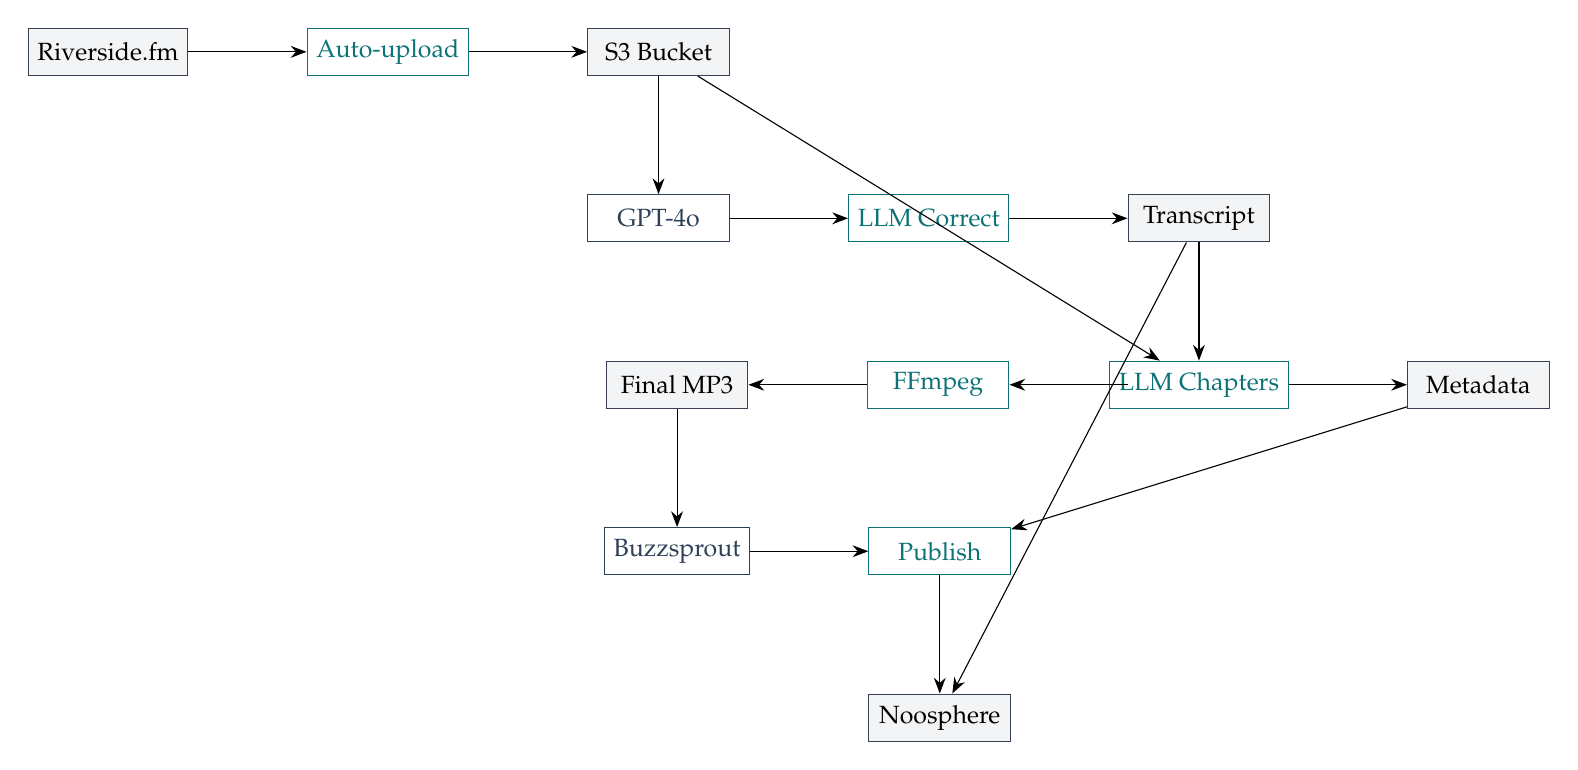
\begin{tikzpicture}[
  node distance=1.2cm and 1.5cm,
  box/.style={
    rectangle,
    draw=darkgray,
    fill=lightgray,
    minimum width=1.8cm,
    minimum height=0.6cm,
    align=center,
    font=\small
  },
  action/.style={
    box,
    fill=white,
    draw=teal,
    text=teal
  },
  service/.style={
    box,
    fill=white,
    draw=accent,
    text=accent
  }
]

% Tier 1: Recording
\node[box] (riverside) {Riverside.fm};
\node[action, right=of riverside] (s3upload) {Auto-upload};
\node[box, right=of s3upload] (s3) {S3 Bucket};

% Tier 2: Transcription
\node[service, below=1.5cm of s3] (transcribe) {GPT-4o};
\node[action, right=of transcribe] (correct) {LLM Correct};
\node[box, right=of correct] (transcript) {Transcript};

% Tier 3: Processing
\node[service, below=1.5cm of transcript] (auphonic) {Auphonic};
\node[action, left=of auphonic] (ffmpeg) {FFmpeg};
\node[box, left=of ffmpeg] (audio) {Final MP3};

% Tier 4: Metadata
\node[action, below=1.5cm of transcript] (chapters) {LLM Chapters};
\node[box, right=of chapters] (metadata) {Metadata};

% Tier 5: Publishing
\node[service, below=1.5cm of audio] (buzzsprout) {Buzzsprout};
\node[action, right=of buzzsprout] (publish) {Publish};

% Tier 6: Knowledge
\node[box, below=1.5cm of publish] (noosphere) {Noosphere};

% Connections
\draw[-{Stealth[length=2mm]}] (riverside) -- (s3upload);
\draw[-{Stealth[length=2mm]}] (s3upload) -- (s3);
\draw[-{Stealth[length=2mm]}] (s3) -- (transcribe);
\draw[-{Stealth[length=2mm]}] (transcribe) -- (correct);
\draw[-{Stealth[length=2mm]}] (correct) -- (transcript);
\draw[-{Stealth[length=2mm]}] (s3) -- (auphonic);
\draw[-{Stealth[length=2mm]}] (auphonic) -- (ffmpeg);
\draw[-{Stealth[length=2mm]}] (ffmpeg) -- (audio);
\draw[-{Stealth[length=2mm]}] (transcript) -- (chapters);
\draw[-{Stealth[length=2mm]}] (chapters) -- (metadata);
\draw[-{Stealth[length=2mm]}] (audio) -- (buzzsprout);
\draw[-{Stealth[length=2mm]}] (metadata) -- (publish);
\draw[-{Stealth[length=2mm]}] (buzzsprout) -- (publish);
\draw[-{Stealth[length=2mm]}] (publish) -- (noosphere);
\draw[-{Stealth[length=2mm]}] (transcript) -- (noosphere);

\end{tikzpicture}
\end{center}

\subsection{Celery Task Graph}

\begin{center}
\begin{tikzpicture}[
  node distance=2cm,
  task/.style={
    ellipse,
    draw=accent,
    fill=white,
    text=accent,
    minimum width=1.5cm
  }
]

\node[task] (watch) {watch\_s3};
\node[task, below=of watch] (transcribe) {transcribe};
\node[task, below=of transcribe] (correct) {correct\_vocab};
\node[task, below=of correct] (cleanup) {cleanup\_audio};
\node[task, below left=of cleanup] (chapters) {generate\_chapters};
\node[task, below right=of cleanup] (publish) {publish};
\node[task, below=of publish] (ingest) {ingest\_noosphere};

\draw[-{Stealth[length=2mm]}] (watch) -- (transcribe);
\draw[-{Stealth[length=2mm]}] (transcribe) -- (correct);
\draw[-{Stealth[length=2mm]}] (correct) -- (cleanup);
\draw[-{Stealth[length=2mm]}] (cleanup) -- (chapters);
\draw[-{Stealth[length=2mm]}] (cleanup) -- (publish);
\draw[-{Stealth[length=2mm]}] (chapters) -- (publish);
\draw[-{Stealth[length=2mm]}] (publish) -- (ingest);

\end{tikzpicture}
\end{center}

\vspace{12pt}

\section{Critical Gaps and Honest Limitations}

\subsection{No Single Platform Covers Everything}

The closest end-to-end path is Descript + SquadCast + Buzzsprout, but even this requires manual filler-word removal in the Descript UI. A fully automated pipeline requires custom integration of 4–6 services.

\subsection{Filler Word Removal}

Filler word removal is the hardest step to automate. Descript does it excellently but has no API for it. A transcript-guided FFmpeg approach works but is cruder. For a philosophical podcast where not every "um" needs surgical removal, Auphonic's adaptive speaker levelling may be sufficient without explicit filler removal.

\subsection{Recording Start is Manual}

No platform supports fully programmatic recording triggers. The founders press a button (or click "Record" in Riverside). Everything after that can be automated.

\subsection{Philosophical Vocabulary Requires Active Maintenance}

A custom vocabulary file must be maintained and updated as new thinkers and concepts enter the conversation. This is a small but ongoing human task.

\subsection{Human Approval Before Publication}

Even in a fully automated pipeline, a single human checkpoint before episode publication is advisable—listen to a 30-second sample, scan the generated show notes, approve. This prevents the occasional transcription error or audio glitch from going live.

\subsection{Emerging Challenge: Deepfake Audio}

As voice cloning (ElevenLabs, Play.ht) becomes more realistic, there's a potential risk of malicious manipulation. Always ensure that any audio published is authenticated (e.g., signed metadata, blockchain-backed transcript hash).

\vspace{12pt}

\section{Conclusion and Next Steps}

You now have a complete map of the podcast infrastructure landscape as of April 2026. The tools are mature, the APIs are stable, and the costs are low.

\subsection{Recommended Implementation Path for Theseus}

\begin{enumerate}
  \item \textbf{Phase 1 (Week 1–2):} Set up Riverside.fm for remote sessions, configure S3 auto-upload.
  \item \textbf{Phase 2 (Week 3–4):} Integrate GPT-4o Transcribe via API, build vocabulary correction prompt.
  \item \textbf{Phase 3 (Week 5–6):} Wire up Auphonic and FFmpeg for audio assembly.
  \item \textbf{Phase 4 (Week 7–8):} Build LLM-based chapter and metadata generation.
  \item \textbf{Phase 5 (Week 9–10):} Integrate Buzzsprout publishing API.
  \item \textbf{Phase 6 (Week 11–12):} Build Noosphere ingestion bridge; wire into Celery.
  \item \textbf{Phase 7 (Week 13+):} Manual testing, QA, and refinement.
\end{enumerate}

\subsection{Cost at Recommended Configuration}

For 2 episodes per week (104 hours/year):

\begin{center}
\begin{tabular}{lr}
\toprule
\textbf{Component} & \textbf{Annual Cost} \\
\midrule
Riverside.fm & \$0 (OBS + PodTrak) \\
GPT-4o Transcribe & \$37 \\
Auphonic & \$20 \\
LLM metadata & \$25 \\
Buzzsprout & \$144 \\
S3 storage & \$15 \\
\midrule
\textbf{Total} & \textbf{\$241} \\
\bottomrule
\end{tabular}
\end{center}

This is remarkably affordable for a production system that handles everything from recording to publishing to knowledge graph ingestion.

\vspace{12pt}

\begin{center}
\rule{0.5\linewidth}{0.5pt}
\end{center}

\vspace{6pt}

\noindent\textit{Theseus Intellectual Capital Partners · Internal Research Document · April 2026}

\end{document}
